\documentclass[conference]{../IEEEtran}

\usepackage{graphicx}
\usepackage{amsmath}
\usepackage{amssymb}
\usepackage{algorithm}
\usepackage{subfigure}
\usepackage{algpseudocode}
\usepackage{multirow}
\usepackage{pdfsync}
\usepackage{siunitx}
\usepackage[]{url}

\providecommand{\e}[1]{\ensuremath{\times 10^{#1}}}

\begin{document}

\title{Lab 2: Odometry Localization}
\author{Yukun Lin and Jennifer Zheng}
\bstctlcite{IEEEexample:BSTcontrol}
\maketitle

\begin{abstract}
  For a wheeled robot, odometry based on wheel rotation and a kinematic model can be used
  as a method of estimating motion and localization. However, errors in odometry
  measurements not accounted by a kinematic model, such as wheel slip caused by different
  coefficient of friction, leads to an accumulation of unbounded error in the motion and
  location estimate over time.  In this paper, we performed experiments to characterize
  the odometry error in the $(x, y)$ position, and heading $\theta$ of a wheeled robot called the
  Jaguar Lite Autonomous Vehicle. Based on a linear regression analysis, the $x$ and
  $\theta$ errors, with respect to actual $x$ displacement, had statistically significant
  slopes and fit values of $R^2>0.90$. These values indicate systematic errors present,
  which can be corrected for in the odometry model.
\end{abstract}

\section{Introduction}
Odometry is a method for calculating the change in the position of a robot based on motion
sensor measurements. This enables the robot to localize itself by successively adding its
measured change in position to its previous position.

One method of odometry counts the number of rotations of a wheel to determine its
displacement. The error from each measurement of a wheel rotation translates to an error
in the estimate of the robot's position. Furthermore, this position error accumulates over
time and is unbounded. Errors from odometry of a wheeled robot can be caused by factors
like the resolution of the sensor used, inaccurate measurements of the wheel diameter, and
varying properties of the surface traveled on. By quantifying these errors through
experimentation, the accuracy of odometry can be improved.

In this paper, we performed experiments to characterize the odometry error of a wheeled
robot called the Jaguar Lite Autonomous Vehicle. Based on these results, we modeled the
odometry error and compensated for it.

\begin{figure*}[t]
  \centering
  \subfigure[]{\includegraphics[width = 6cm]{figures/JaguarLabel.pdf}
  \label{fig:jag}}
  \hspace{0.5cm}
  \subfigure[]{\includegraphics[width = 4.5cm]{figures/encoder.pdf}
  \label{fig:encoder}}
  \subfigure[]{\includegraphics[width = 5.6cm]{figures/encoderDigital.pdf}
    \label{fig:encoderDig}}
  \caption{The Jaguar Lite Autonomous Vehicle used is shown in Fig.~\ref{fig:jag}.
           An illustration of an incremental encoder is shown in Fig.~\ref{fig:encoder}
           and the digital output of the encoder is shown in Fig.~\ref{fig:encoderDig}
           \cite{jag, encoders, detector}.}
  %http://irobotec.com/shop/defense-security-surveillance-robots/jaguar-lite-platform/
  %http://mechatronics.mech.northwestern.edu/design_ref/sensors/encoders.html

  %http://www.pittman-motors.com/Gearboxes-Brakes-Encoders/Encoders/H-Series-Incremental-Encoder.aspx
\end{figure*}

\section{Background}
%Jennifer
The Jaguar is a wheeled robot that is track driven and developed by Dr. Robot Inc. It  can
operate on rough terrains and is equipped with outdoor GPS, a 9-DOF IMU, a high-resolution
video camera, and a laser scanner.

The wheel rotations of the robot are calculated using incremental encoders. The encoder includes a transparent disk with black lines painted on it. A diagram of the encoder is shown in Fig.~\ref{fig:encoder}. The photoemitter on the encoder emits a light; this light passes through the disk to on the clear lines and is blocked on the black lines. The phototransistor outputs a high or low signals based on the detection of the emitted
light, as shown in Fig.~\ref{fig:encoderDig}.
The Jaguar's encoder can count up to 32767 before rolling over. A full rotation
of the wheel results in 190 pulses from the encoder.

\begin{figure*}[t]
  \centering
  \subfigure[]{\includegraphics[width = 6cm]{figures/KinAxis.png}
  \label{fig:kinAxis}}
  \subfigure[]{\includegraphics[width = 4cm]{figures/kinAngle.png}
  \label{fig:kinAngle}} \hspace{1.5cm}
  \subfigure[]{\includegraphics[width = 5cm]{figures/kinXY.png}
  \label{fig:kinXY}}
  \caption{Initial kinematics diagram showing the global coordinate frame is shown in
           Fig.~\ref{fig:kinAxis}. Kinematics model with angle measurements is shown in
           Fig.~\ref{fig:kinAngle}. Kinematics model labeled with $\Delta x$ and $\Delta y$.
           is shown in Fig.~\ref{fig:kinXY} \cite{lecture}.}
\end{figure*}

\section{Kinematics Model}
The Jaguar is modeled as a two-wheeled robot,
with wheels of radius $r$ and a distance of $2L$ between its left and right wheels. The kinematics model is shown in Fig.~\ref{fig:kinAxis}. It is used to determine the robot's change in position and heading based on odometry measurements. Given the robot's initial pose, the change in the robot's position and heading determines the robot's subsequent state in the global coordinate frame.

\subsection{Displacement and Rotation}

The distance traveled by the left and right wheel is denoted by $\Delta s_l$ and
$\Delta s_r$, and the distanced traveled by the robot is denoted by $\Delta s$.
The relationship between $(\Delta s_l, \Delta s_r)$ and $\Delta s$ is illustrated in
Fig.~\ref{fig:kinAngle}. The distance traveled by the left and right wheel is calculated
using encoder readings as shown in Alg.~\ref{alg:rotation}.

\begin{algorithm}[b]
  \caption{Wheel Distance Traveled}
  \begin{algorithmic}[1]
    \Function{GetDistance}{$z_{enc}^{t-1}$}
      \State $\Delta z_{enc}^{t} \gets z_{enc}^{t-1} - z_{enc}^{t}$
      \medskip
      \If{$|\Delta z_{enc}^{t}| > \text{encoderMax} / 2$}
        \If{$\Delta z_{enc}^{t} < 0$}
          \State $\Delta z_{enc}^{t} \gets \Delta z_{enc}^{t} + \text{encoderMax}$
        \Else
          \State $\Delta z_{enc}^{t} \gets \Delta z_{enc}^{t} - \text{encoderMax}$
        \EndIf
      \EndIf
      \medskip
      \State $f \gets \Delta z^{t}_{enc} / T_{\text{rotation}}$
      \medskip
      \State \Return $f*2\pi *r$
    \EndFunction{}

    \end{algorithmic}
  \label{alg:rotation}
\end{algorithm}

The encoder pulse value at time $t$ is denoted by $z_{enc}^t$, and
the difference between the current and previous encoder pulse values denoted by $\Delta z_{enc}^t$
is first calculated (Alg.~\ref{alg:rotation}, line 2).
Rollover in the encoder value is checked and corrected for (Alg.~\ref{alg:rotation}, line 3-9).
The fraction of wheel rotation, $f$, is then calculated (Alg.~\ref{alg:rotation}, line 10), where
$T_{\text{rotation}}$ is the number of encoder pulse value in one full wheel rotation.
The distance traveled by the wheel is then calculated by multiplying wheel rotation count by
the circumference of the wheel (Alg.~\ref{alg:rotation}, line 11).

The distance traveled by the robot is the average of the distance traveled by the left and
right wheel and is given by
\begin{equation}
  \Delta s = \frac{\Delta s_r+\Delta s_l}{2},
  \label{eq:midDist}
\end{equation}
and the rotation of the robot is proportional to the difference between the distance
traveled by the left and right wheel and is given by
\begin{equation}
  \Delta \theta = \frac{\Delta s_r-\Delta s_l}{2L}.
  \label{eq:deltTheta}
\end{equation}

\subsection{Localization with Odometry}

The distance traveled and rotation of the robot is used to calculate its change in position
$(\Delta x, \Delta y)$ in the global frame; this is illustrated in Fig.~\ref{fig:kinXY}.
Assuming that the motion between each odometry update is small enough,
it follows that $\Delta d \approx \Delta s$. The change in robot position is therefore given by Eq.~\ref{eq:deltX} and Eq.~\ref{eq:deltY}.
%
\begin{align}
  \Delta x &=
  \Delta d \cos{(\theta+\Delta\theta/2)} \approx \Delta s \cos{(\theta+\Delta\theta/2)}
  \label{eq:deltX}\\
  \Delta y &=
  \Delta d \sin{(\theta+\Delta\theta/2)} \approx \Delta s \sin{(\theta+\Delta\theta/2)}
  \label{eq:deltY}
\end{align}

The current robot position and heading can be calculated by adding $(\Delta x, \Delta y)$ and
$\Delta \theta$ to the previous robot position and heading respectively.

\section{Experiments}
Experiments to characterize the error in odometry was conducted in Parsons Engineering
Building and outside of the Sprague Learning Center. Two locations with different floor surfaces,
smooth tiles and concrete respectively, were chosen to compare the effect of floor surface on odometry error. At each location, two sets of trials were conducted.

\begin{figure}[h] \centering
  \subfigure[]{\includegraphics[width=4.2cm]{figures/straight_line.pdf}
  \label{fig:line_test}}
  \subfigure[]{\includegraphics[width=4.2cm]{figures/rotation.pdf}
  \label{fig:rotation_test}}
  \caption{The setup for the straight line tests and rotation tests are shown in
           Fig.~\ref{fig:line_test} and Fig.~\ref{fig:rotation_test} respectively.}
\end{figure}

\begin{figure*}[t]
  \centering
  \subfigure[]{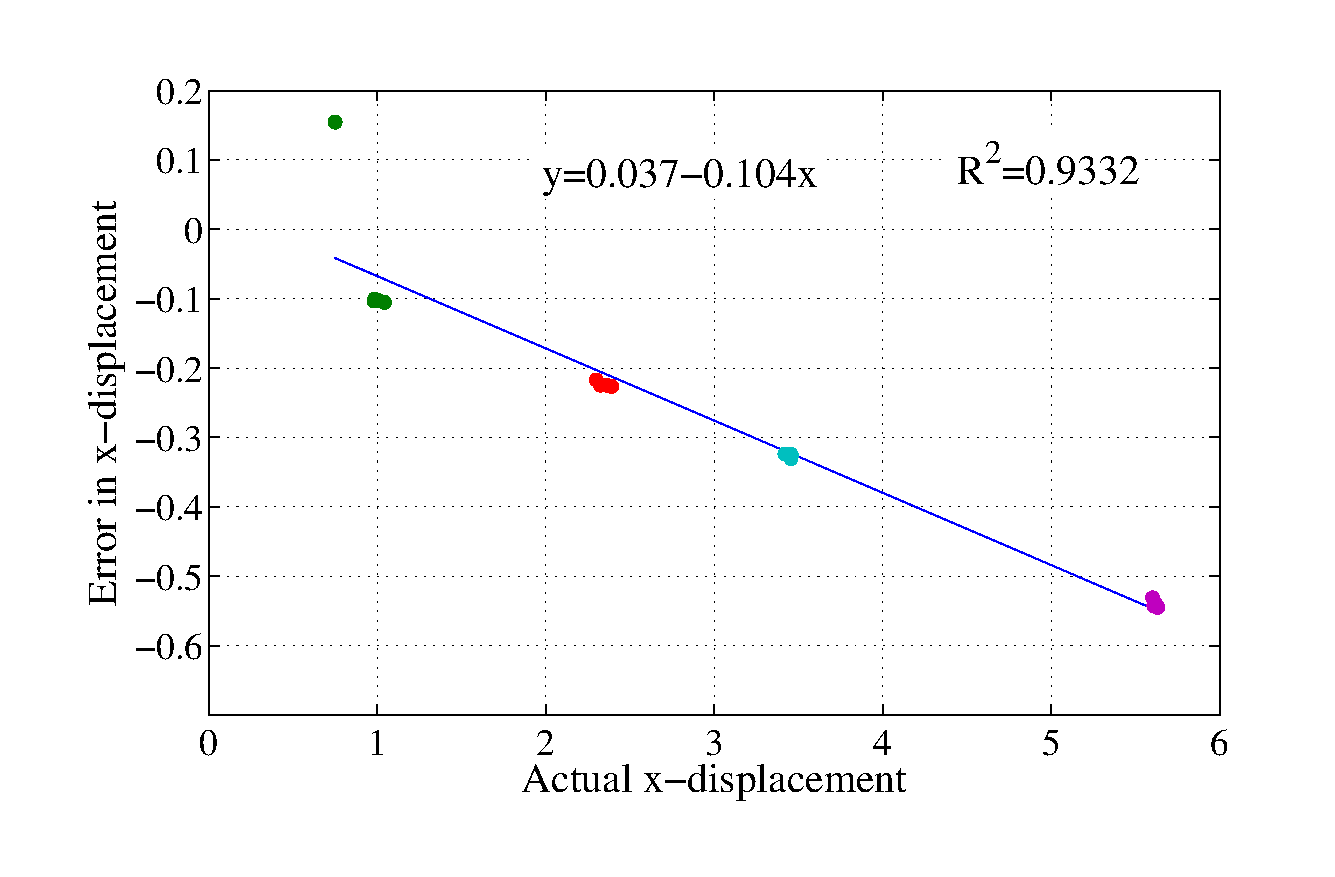
\includegraphics[width = 5.8cm]{figures/tile_xError.eps}
  \label{fig:tileX}}
  \subfigure[]{\includegraphics[width = 5.8cm]{figures/tile_yError.eps}
  \label{fig:tileY}}
  \subfigure[]{\includegraphics[width = 6.15cm]{figures/theta_vs_err_basement.pdf}
  \label{fig:theta_basement}}

  \subfigure[]{\includegraphics[width = 5.8cm]{figures/concrete_xError.eps}
  \label{fig:concreteX}}
  \subfigure[]{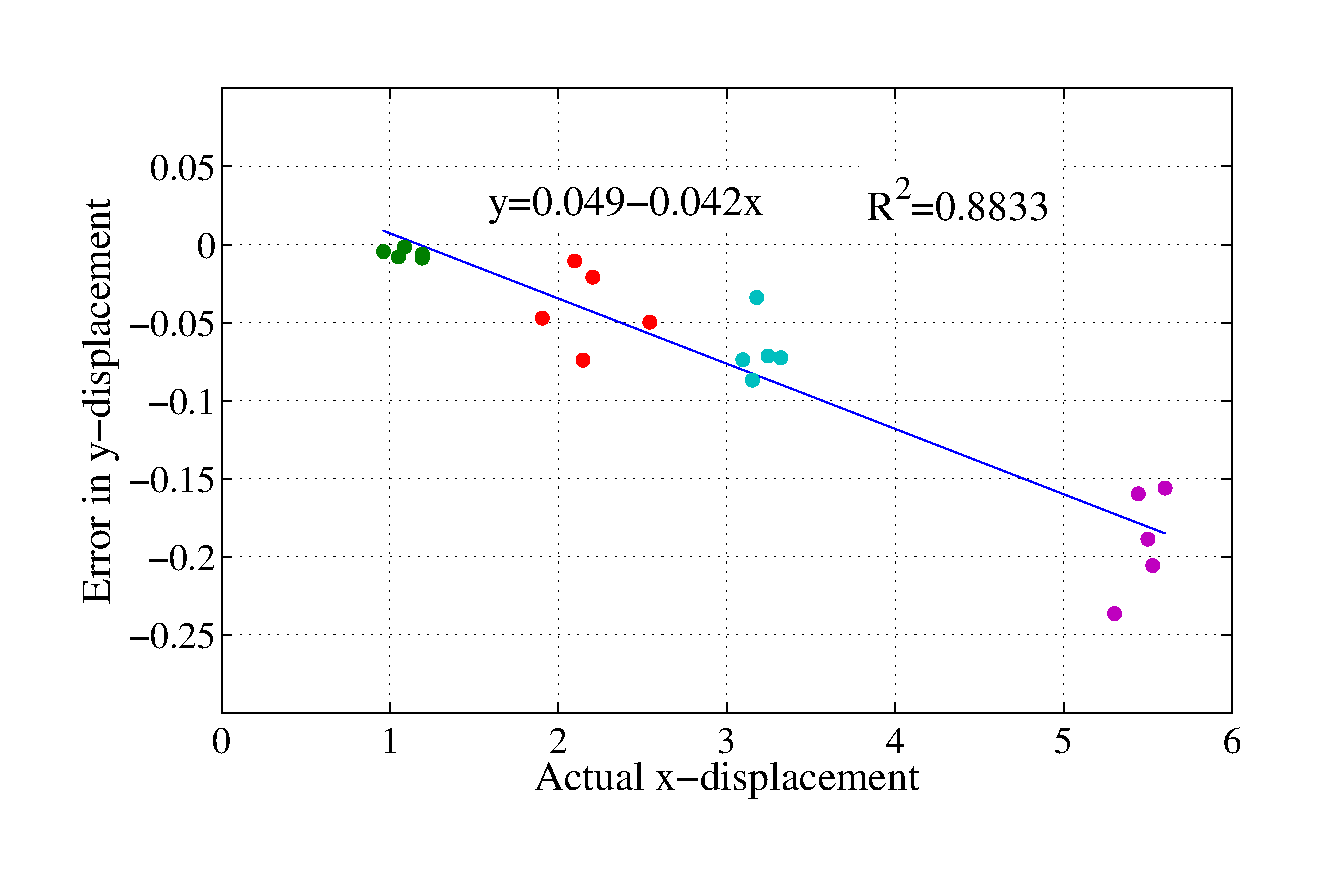
\includegraphics[width = 5.8cm]{figures/concrete_yError.eps}
  \label{fig:concreteY}}
  \subfigure[]{\includegraphics[width = 6.15cm]{figures/theta_vs_err_concrete.pdf}
  \label{fig:theta_concrete}}

  \caption{The $x$, $y$ and $\theta$ errors for trials conducted on smooth tile as
           a function of actual displacement and rotation are
           shown in Fig.~\ref{fig:tileX}, Fig.~\ref{fig:tileY}, and Fig.~\ref{fig:tileY}
           respectively. The same errors for trials conducted on concrete are shown in
           Fig.~\ref{fig:concreteX}, Fig.~\ref{fig:concreteY}, and Fig.~\ref{fig:theta_concrete}.}
  \label{fig:odo_errors}
\end{figure*}

\subsection{Design}

The first set of trials is referred to as the \emph{Straight Line Tests}.
The Jaguar was driven forward in a straight line for distances of approximately
\SI{1}{\meter}, \SI{2}{\meter}, \SI{3}{\meter}, and \SI{5}{\meter} as estimated by odometry.
The actual $x$ and $y$ displacements was also measured. For these set of trials, a global
coordinate frame with axis $X_I$ and $Y_I$ was established, as shown in
Fig.~\ref{fig:line_test}. The robot's initial starting position was at the
origin of the global frame, with a heading parallel to the global $x$ axis.

The second set of trials is referred to as the \emph{Rotation Tests}. The same global
coordinate frame from the straight line tests was used. The Jaguar rotated on the spot
with angles of rotation of approximately \SI{45}{\degree}, \SI{90}{\degree},
\SI{-45}{\degree}, and \SI{-90}{\degree}. The angle of rotation with respect to $X_I$ was
then determined trigonometrically, as shown in Fig.~\ref{fig:rotation_test}. This was
repeated five times for each angle of rotation.

\subsection{Straight Line Test Alignment}

\begin{figure}[b] \centering
  \subfigure[]{\includegraphics[width=4cm]{figures/initial.jpg}
  \label{fig:jagSetup}}
  \subfigure[]{\includegraphics[width=4cm]{figures/change_measure.jpg}
  \label{fig:jagYerror}}
  \caption{The alignment and measurement setup for the straight line tests are shown in
           Fig.~\ref{fig:jagSetup} and Fig.~\ref{fig:jagYerror} respectively.}
\end{figure}

The Jaguar was aligned for the straight line tests using blue tape to mark its initial
position and change in position, as seen in Fig.~\ref{fig:jagSetup}.
Fig.~\ref{fig:jagYerror} shows how the $y$ displacement was found by measuring the
distance between the blue tape center line and blue tape on the robot. The $x$
displacement was found by measuring the distance between the initial starting and final
robot position.

\section{Results and Discussions}

\subsection{Straight Line Tests}

The odometry errors in $x$ and $y$ position of the straight line tests are presented in
Fig.~\ref{fig:odo_errors}. Here, error is defined as
%
\begin{equation}
x_{\text{error}} = x_{\text{odometry}} - x_{\text{measured}}.
\label{eq:error}
\end{equation}
%
Three general trends were observed in the error plots. For both the concrete and tile
tests, the $x$ error was biased to the negative $x$ direction as illustrated in
Fig.~\ref{fig:concreteX} and Fig.~\ref{fig:tileX}. In addition, the error in the $x$
direction was larger than in the $y$ direction. Finally, the $x$ and $y$ odometry in the
error tends to increase in magnitude with respect to actual $x$ displacement.

%Yukun
\subsection{Rotation Tests}

The odometry errors in the rotations tests are presented in Fig.~\ref{fig:theta_basement}
and Fig.~\ref{fig:theta_concrete}.  Here, heading error is defined as
%
\begin{equation}
  \theta_{err} = \theta_{\text{odometry}} - \theta_{\text{measured}}.
\end{equation}
%
Fig.~\ref{fig:theta_basement} and Fig.~\ref{fig:theta_concrete} shows that for all trials,
the odometry over-estimates the rotation that happened; in addition, the magnitude of
heading error increases with the magnitude of the rotation.

\begin{table*}[t] \centering
  \caption{Linear regression parameters of $x$, $y$, and $\theta$ error.}
  \begin{tabular}{| c | c | c | c | c | c | c | c | c |}
    \hline
    \multirow{2}{*}{} &
    \multicolumn{4}{c|}{Smooth Tile} &
    \multicolumn{4}{c|}{Concrete} \\ \cline{2-9}
    & Slope & Intercept & $R^2$ & P-value & Slope & Intercept & $R^2$ & P-value \\ \hline
    $x$ error      & -0.104   & 0.0365  & 0.933  & 5.04\e{-17}
                   & -0.0880  & 0.00251 & 0.999  & 1.13\e{-27} \\ \hline
    $y$ error      & -0.00384 & 0.0200  & 0.0285 & 0.477
                   & -0.0418  & 0.0490  & 0.883  & 7.90\e{-10} \\ \hline
    $\theta$ error & 0.283    & -2.11   & 0.937  & 2.94\e{-12}
                   & 0.247    & -3.45   & 0.918  & 3.40\e{-11} \\ \hline
  \end{tabular}
  \label{table:straight}
\end{table*}

\begin{figure*}[t]
  \centering
  \subfigure[]{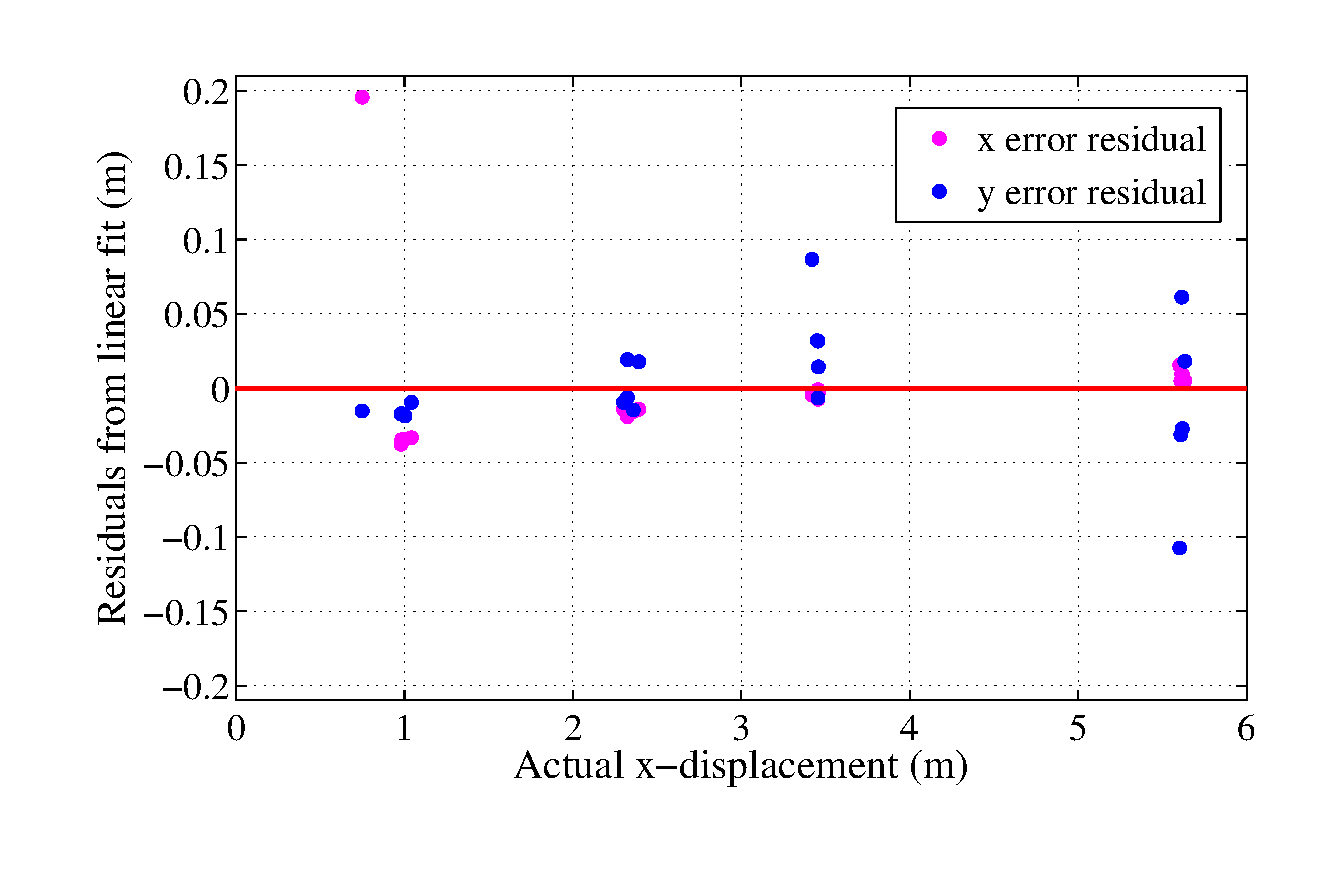
\includegraphics[width = 5.8cm]{figures/tile_residual.eps}
  \label{fig:tileRes}}
  \subfigure[]{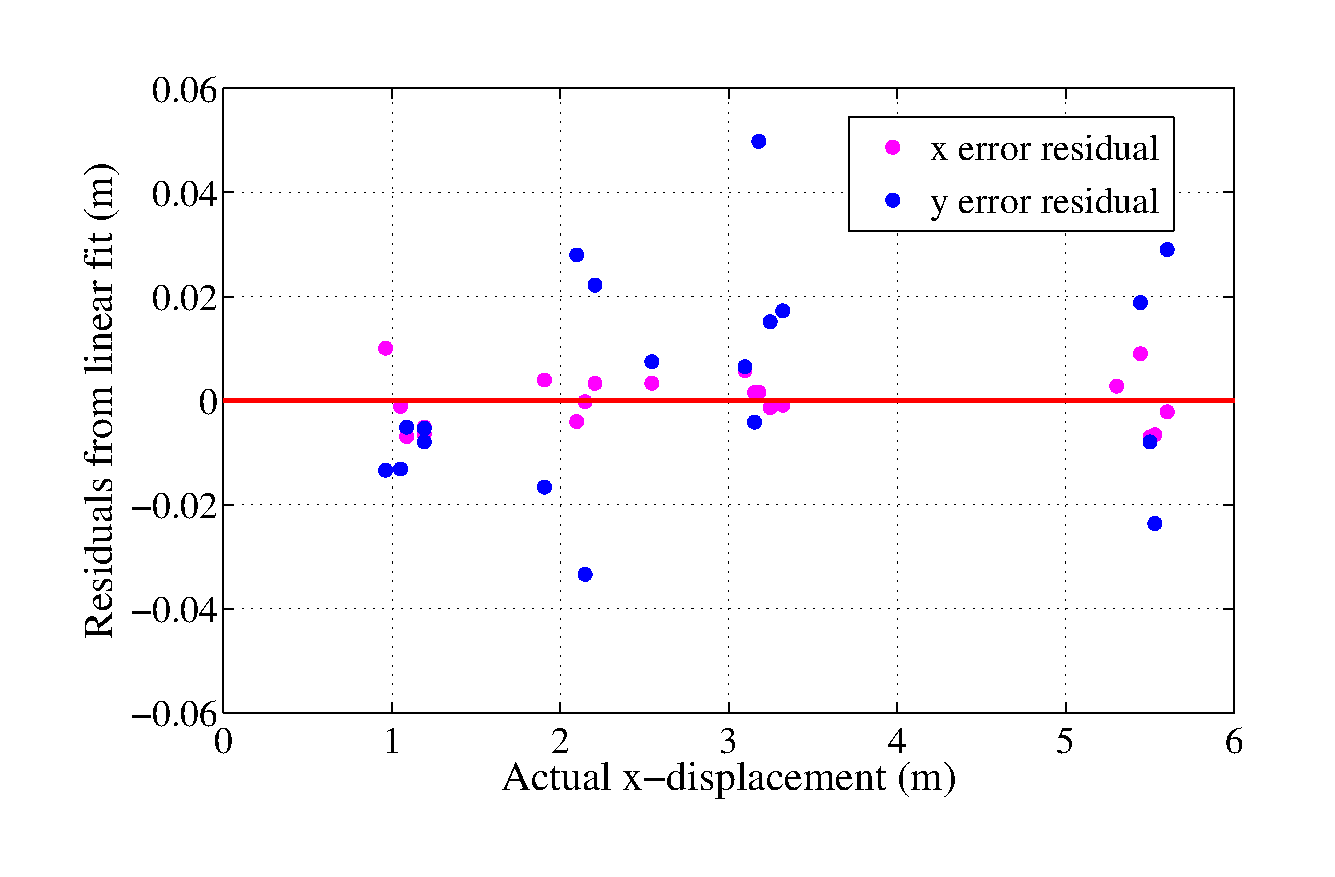
\includegraphics[width = 5.8cm]{figures/concrete_residuals.eps}
  \label{fig:conRes}}
  \subfigure[]{\includegraphics[width = 6.15cm]{figures/theta_res.pdf}
  \label{fig:thetaRes}}
  \caption{The residual plots from the linear regression fits on the odometry error.
           The $x$ and $y$ residuals for the concrete tests are shown in (a) and the
           residuals for the tile tests are shown in (b).}
  \label{fig:residuals}
\end{figure*}

\subsection{Linear Regression Analysis}
The error plots in Fig.~\ref{fig:odo_errors} exhibit a linear trend; thus a linear
regression model was used and plotted with the data points. Fig.~\ref{fig:residuals} shows
the residual plots of the linear regressions. Most of the residual plots show a random
scattering of data points.

However, for the straight line tests on tile, residuals for the $x$ errors shown in
Fig.~\ref{fig:tileRes} exhibit a linear trend. This trend indicates that the slope of the
least-square fit does not best model this trend. However, this does not imply that a
linear fit is not appropriate for the data.  On closer observation, there is an outlier in
the corresponding data set, as seen in Fig.~\ref{fig:tileX}. This outlier biases the slope
of the least-square fit, causing the linear trend observed in the residuals.

%%%%%%%%%%%%%%%%%%added%%%%%%%%%%%%%%%%%
The tests between the concrete and tile floors show some difference in slope of the $x$
error best-fit and $\theta$ error best-fit. For the $\theta$ error, the slope difference
between the two floors is $0.036$. For the $x$ error, the slope difference is $0.016$.
This value would be smaller if the regression for the tile tests did not include the
outlier from the \SI{1}{m} test. In addition, the data cannot determine whether the slope
differences between the floors is a direct result of the floor properties.

%%%%%%%%%%%%%%%%%%%%%%%%%%%%%%%%%%%%%%%
Table~\ref{table:straight} summarizes the parameters of the fit and their significance.
All the fits show statistically significant slopes with the exception of the fit for the
$y$ error on tile. The table shows that for the $y$ error on the smooth tile, there is no
statistically significant correlation between the actual $x$ displacement and $y$ error.
Even though the Table~\ref{table:straight} shows that the slope for the $y$ error on
concrete is statistically significant, observing the magnitude of the slope, the $y$ error
in the odometry calculations are negligible for $x$ displacements less than
\SI{2}{\meter}. Note, this error is unbounded over an extended distance. The slopes of
least-square fits of the $x$ and rotation errors on both concrete and tile indicate
systematic errors.

\subsection{Systematic Error}

Slipping is a likely cause of the systematic error for rotation. The kinematic model used
does not account for slipping, therefore the odometry will overestimate the rotation, as
seen in Fig.~\ref{fig:theta_basement} and Fig.~\ref{fig:theta_concrete}. In addition, this
matches the observation that slipping occurred during the rotation tests. Slipping can be
caused by variable friction between the ground and the track. This was observed when a
constant power was applied to the motors but the rotation of the Jaguar was not smooth.

\begin{figure}[t] \centering
  \includegraphics[width=6cm]{figures/wheel.jpg}
  \label{fig:wheel}
  \caption{Under-estimation of the wheel radius. The radius of the wheel
           used did not account for the thickness of the track.}
\end{figure}

Similarly, slipping likely contributed to systematic error in the straight line trials.
Slipping of the tracks happen when the Jaguar starts moving. However, the more likely
source of systematic error comes from an inaccurate measurement of the wheel radius. The
diameter of the inner wheel was measured, as pictured in Fig.~\ref{fig:wheel}. However,
the actual radius includes the treads on the outside on the outside of the wheel. From
Alg.~\ref{alg:rotation} line 11 and Eq.~\ref{eq:midDist}, a smaller radius would result in
a smaller change in position. This is consistent with the negative sloping $x$ error in
both Fig.~\ref{fig:tileX} and Fig.~\ref{fig:concreteX}.

Underestimating the wheel radius also affects the heading estimates, as it would lead to
an underestimation of $\Delta \theta$ as shown by Eq.~\ref{eq:deltTheta}.  However, the
positive trend in Fig.~\ref{fig:theta_basement} and Fig.~\ref{fig:theta_concrete} suggests
that the effect of wheel radius on heading estimate is smaller relative to the effect of
slipping.

\subsection{Random Error}

Random errors in odometry measurements also contributes to error in the position and
heading estimates. These types of error may come from properties of the surface. The
concrete floor and tile floor where the trials have different degrees of smoothness and
coefficients of friction. For example, bumps and cracks in the concrete may affect the
odometry measurements. Furthermore, the kinematic model assumes the behavior in the left
and right wheels are the same. However, the coefficient of friction between the right
wheel and the surface and the left wheel and the surface may be different, thus affecting
position and heading estimates.

\addtolength{\textheight}{-14.5cm}

\subsection{Measurement Error}

Another source of position and heading errors could be errors in the
experimental setup. These errors include slight variation in the starting
position and heading of the robot. For example, if the initial heading of
the robot was not exactly parallel to the global $x$ axis, it could lead
to movement of the robot in the $y$ direction and contribute to $y$ position
error.

For the concrete test trials, the layout of the floor may have affected the
robot's movements. The flooring is composed of an array of cement squares,
with gaps in between each square. For the straight line concrete tests, the
Jaguar was aligned with the edge of a concrete square. The Jaguar consistently
drove into these gaps. This may have restricted the robot's movements from
further moving in the $y$ direction, thus bounding the $y$ displacement error.

\section{Conclusion}
This report presents test methods, test results, and linear regression models that
characterize odometry error of the Jaguar. Based on the regression analysis, the $x$ and
$\theta$ error slope for concrete and tile was statistically significant and had a fit of
$R^2>0.90$, indicating the presence of systematic error.

The systematic error in $\theta$ most likely came from slipping, which was not accounted
for in the kinematics model. This is consistent with test observations where the robot did
not rotate smoothly and test results where the odometry consistently measured above the
actual $x$ value. For $x$, the systematic error likely resulted from an inaccurately
measured wheel radius. The radius used in the odometry algorithm was smaller than its
actual value. This corresponds to a smaller calculated change in $\Delta x$ and $\Delta
y$, which is consistent with the $x$ odometry values being consistently smaller than the
measured $x$ displacement.

Tests were performed on two different surfaces to compare the effect of floor properties
on odometry error. The $x$ error best-fit slope for tile was -0.104, while the best-fit
slope for concrete was -0.088. Because the tile floor has a lower coefficient of friction,
more slipping may have occurred during the tile tests, which would account for the tile's
greater magnitude slope. However, this relationship cannot be attributed to floor
properties because of many uncontrolled variables and error sources in the experiment.

Based on these results, the simple kinematics model used for odometry provides a basis for
localization. However, error characterization can provide corrections to the model to make
the odometry more accurate.

\nocite{*}
\bibliographystyle{ieeetran}
\bibliography{citations}

\end{document}
